\documentclass[10pt, xcolor=dvipsnames]{beamer}
%\documentclass[10pt, xcolor=dvipsnames,notes=only]{beamer}
%\mode<presentation>
%{
\usetheme{Goettingen}
%\setbeamercovered{transparent}
%} 
\usefonttheme{professionalfonts}
%\usecolortheme{beaver}

\usepackage{setspace}
\usepackage[english]{babel}
\usepackage[latin1]{inputenc}
\usepackage{times}
\usepackage[T1]{fontenc}
\usepackage{color}
\usepackage{graphicx}
\usepackage{amssymb}
\usepackage{amsthm}
\usepackage{bm}
\usepackage{rotating}
\usepackage{ccaption}
\usepackage{booktabs}
\usepackage{lscape}
\usepackage{colortbl}
\usepackage{arydshln}
\usepackage{tabularx}
\usepackage{graphics}
\usepackage{epstopdf}

\setbeamertemplate{navigation symbols}{}
\setbeamertemplate{items}[balls]

\newenvironment{changemargin}[2]{%
  \begin{list}{}{%
    \setlength{\topsep}{0pt}%
    \setlength{\leftmargin}{#1}%
    \setlength{\rightmargin}{#2}%
    \setlength{\listparindent}{\parindent}%
    \setlength{\itemindent}{\parindent}%
    \setlength{\parsep}{\parskip}%
  }%
  \item[]}{\end{list}}

\setbeamercolor{block title}{fg=white, bg=teal}
\setbeamercolor{block body}{bg=teal!25}

\author[]{Chad Jones and Dietrich Vollrath}
\institute[Intro Growth]{Introduction to Economic Growth}
\date[]{}


\title[Future]{The future of growth}


\begin{document}
\maketitle

\section{The long-run growth rate}
\begin{frame}{Historical versus long-run}
We've used data on historical growth, but that need not be the same as long-run growth.
\begin{itemize}
	\item Historical growth includes lots of transitions
	\item Convergence via physical capital accumulation
	\item Catch-up growth via diffusion and adoption of technologies
	\item Transitory growth via changes in education, R\&D, and energy use
\end{itemize}
What is the underlying long-run rate of growth from the sense of Romer/Schumpterian set-up?
\end{frame}

\begin{frame}{Production}
Let GDP per capita be determined by
\begin{equation}
	y_t = \left(\frac{K_t}{Y_t}\right)^{\alpha/(1-\alpha)} A_t h_t \frac{L_t}{N_t}, \nonumber
\end{equation}
so that the growth rate is
\begin{equation}
	g_y = \frac{\alpha}{1-\alpha}g_{KY} + g_A + g_h + g_{LN}. \label{EQ_gy_longrun}
\end{equation}
\end{frame}

\begin{frame}{Long-run growth}
\begin{scriptsize}
\begin{tabular}{lrrrr}
\midrule
            &               & \multicolumn{3}{c}{Long-Run Growth Estimates:} \\ \cmidrule(lr){3-5}
            & Historical    & Baseline   & Lower $\frac{\lambda}{1-\phi}$ & $g_L = 0$ \\
Component   &  (1)          &   (2)      &   (3)    & (4) \\
\midrule
GDP per capita ($g_y$) & \phantom{-}1.98\%  &   0.43\%   &  0.31\%   &  $\approx$ 0\%  \\ \\
Capital/output ($\frac{\alpha}{1-\alpha} g_{KY}$) & -0.15\% & 0\%  &  0\% &  0\% \\
Human capital ($g_{h}$) & \phantom{-}0.55\%   &  0\%  &  0\% & 0\% \\
Labor force ($g_{LN}$) & \phantom{-}0.25\%   & 0\%   &  0\%  & 0\% \\
Productivity ($g_{A}$) & \phantom{-}1.32\%   &  0.43\% & 0.31\%   & 0\% \\ \\
\multicolumn{5}{l}{Productivity breakdown:} \\
--Misallocation &  \phantom{-}0.30\%  &  0\%  &  0\% &  0\% \\
--R\&D intensity ($\frac{\lambda}{1-\phi}g_{sR}$) & \phantom{-}0.63\%  &  0\%  &  0\%  & 0\% \\
--Population ($\frac{\lambda}{1-\phi}g_{L}$) & \phantom{-}0.39\%   & 0.39\%  & 0.28\%  & $\approx$ 0\% \\
\midrule
\end{tabular}
\end{scriptsize}
\end{frame}

\begin{frame}{Long-run growth}
The underlying rate of growth is probably around 0.39\% per year. 
\begin{itemize}
	\item Lots of productivity growth appears to be because of rising $s_R$
	\item Remember that population growth is the ultimate determinant, and it isn't that big?
	\item ``Misallocation'' here refers to improvements in allocations over time via changes in who's allowed to participate in economic activity
\end{itemize}
Most sources of growth could die out because they are inherently transitory. For example, you can't raise the labor force participation rate above 100\%. 
\end{frame}

\section{Demographics}
\begin{frame}{Slow population growth}
The last column considered what happens if $g_L \approx 0$.
\begin{itemize}
	\item The Romer/Schumpeter models tell us $g_A \approx 0$ in this case
	\item The rate at which we increase ideas can't keep up with the size of the stock, $A$
	\item We innovate, but it becomes minor compared to the stock of ideas we already have
\end{itemize}
\end{frame}

\begin{frame}{Demographic change}
\begin{center}
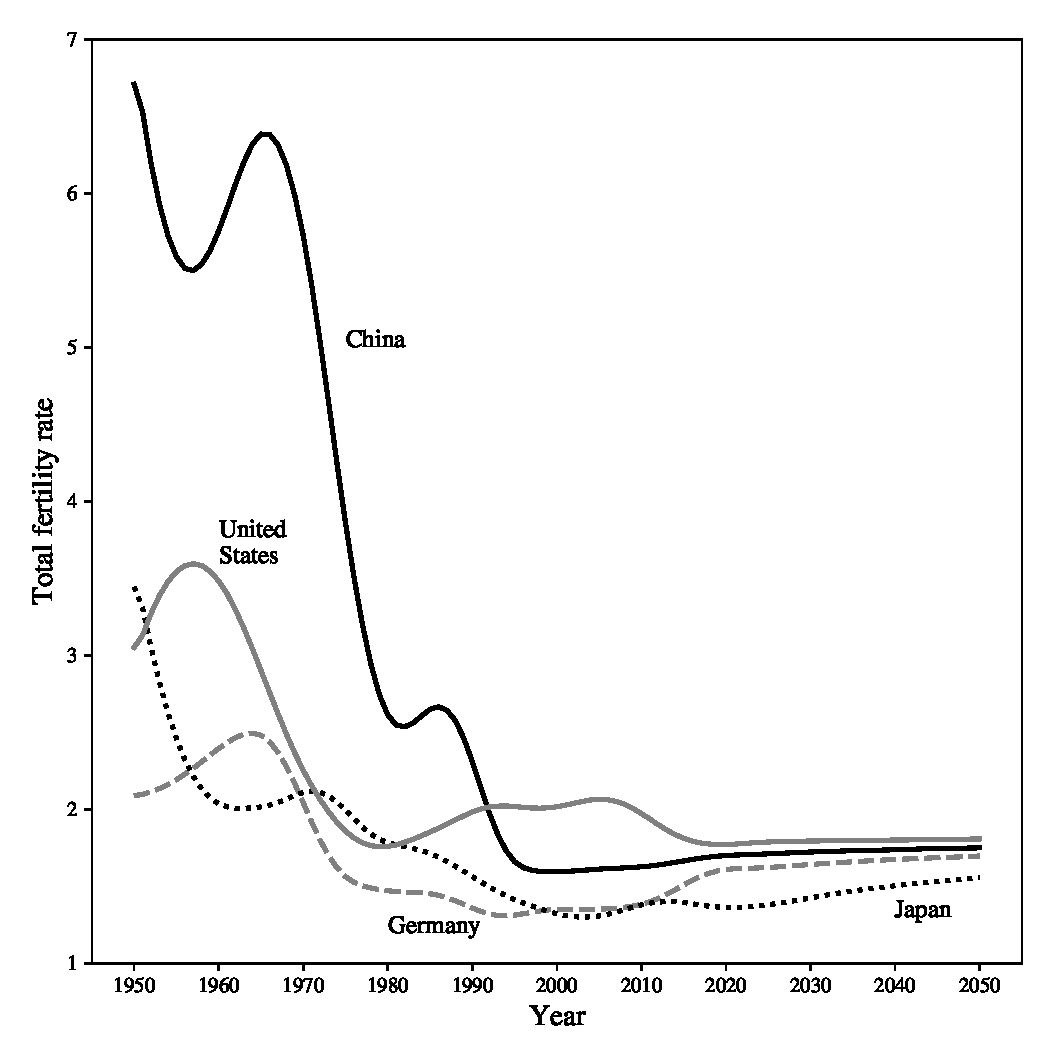
\includegraphics[height=3in]{../Figures/fig-ch12-fig1.eps}
\end{center}
\end{frame}

\begin{frame}{Demographic change}
\begin{center}
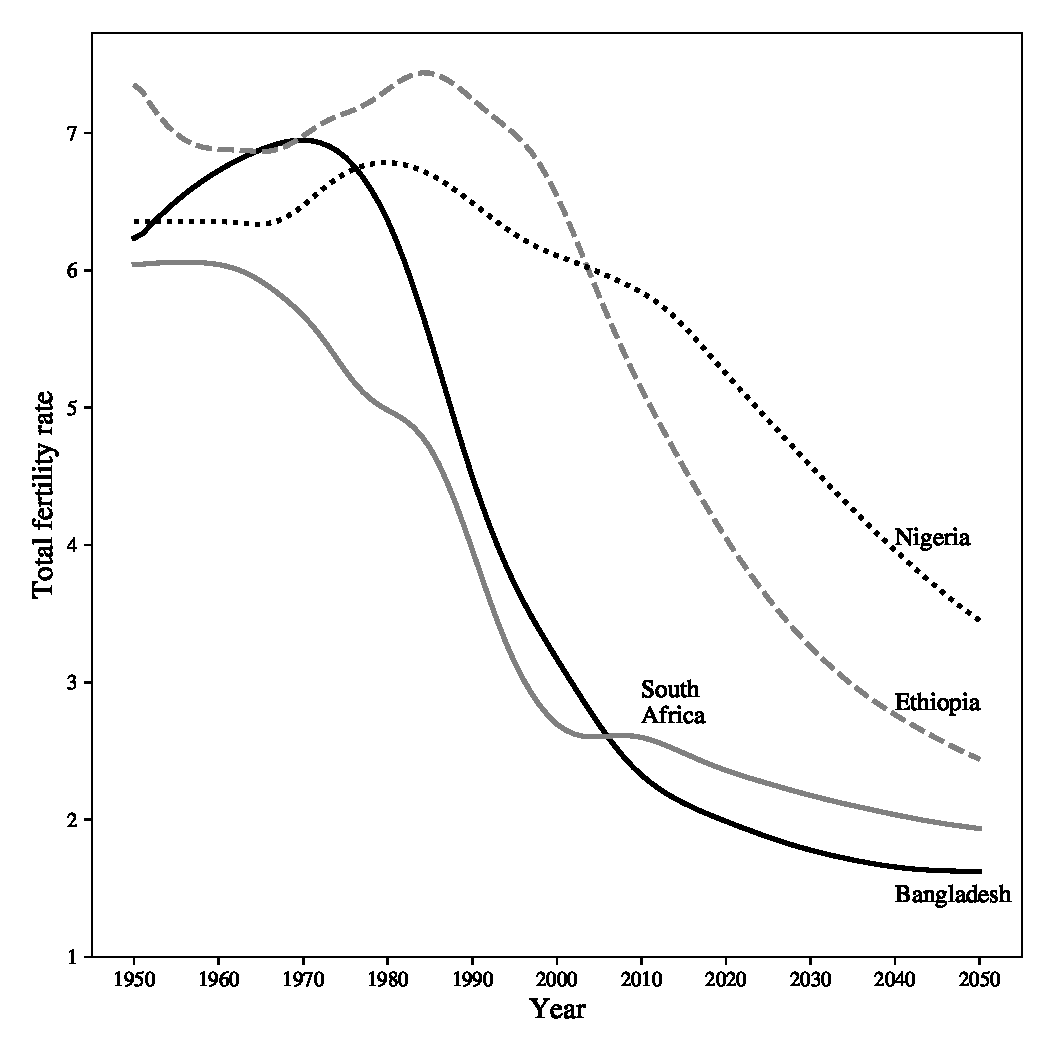
\includegraphics[height=3in]{../Figures/fig-ch12-fig2.eps}
\end{center}
\end{frame}

\begin{frame}{Negative population growth}
What happens if population goes \textit{down} worldwide? From Romer/Schumpeter we have
\begin{equation}
	g_A = \theta \frac{s_R^{\lambda} L_0^{\lambda} e^{\lambda g_L t}}{A_t^{1-\phi}}. \nonumber
\end{equation}
and if $g_L <0$
\begin{itemize}
	\item $e^{\lambda g_L t} = 0$
	\item Innovation just \textit{stops}
	\item New ideas flow so slowly we effectively stagnate
\end{itemize}
\end{frame}

\begin{frame}{Demographic optimism}
Even if overall population growth slows down or reverses, still have innovation?
\begin{itemize}
	\item Vast majority of world does not engage in innovation
	\item Even if population doesn't grow, if you include several billion Africans and Asians in innovation networks, we add to R\&D efforts for centuries
	\item The key is that we care about the number of R\&D workers, which combines $s_R$ and $L$
	\item There is scope to raise worldwide $s_R$ from around zero to 2-3\% 
\end{itemize}
\end{frame}

\section{Automation}
\begin{frame}{Automating production}
Automation has been going on for centuries. New instances like AI may be just another example or a fundamental change. Consider
\begin{equation}
	Y = A X_1^{1/n} X_2^{1/n} ... X_n^{1/n}. \nonumber
\end{equation}
as how we produce GDP. 
\begin{itemize}
	\item Different varieties, like Romer
	\item But we can produce each X using either capital or labor
	\item Let $m$ tasks be done by capital, the other $n-m$ by labor
\end{itemize}
\begin{equation}
	Y = A K^{m/n} L^{1 - m/n}. \label{EQ_Y_mn}
\end{equation}
\end{frame}

\begin{frame}{Automating production}
With
\begin{equation}
	Y = A K^{m/n} L^{1 - m/n}. \label{EQ_Y_mn}
\end{equation}
we are changing the $\alpha$ term in the Solow/Romer. Note that the $A$ here does \textit{not} sit ``inside'' of any terms so
\begin{equation}
 	g_y^{ss} = \frac{g_A}{1-m/n}. \label{EQ_gy_mn}
 \end{equation} 
The larger is $m$ (the more automation) the higher is the growth rate, even given productivity growh. 
\end{frame}

\begin{frame}{Does this make sense?}
If $m$ goes up, this would imply that the share of GDP going to capital rises, but that doesn't appear to be the case in the long-run
\begin{itemize}
	\item It could be that $n$ is expanding (new varieties) just as fast as we automate ($m$ rises)
	\item It could be that tasks are complements, and as $m$ goes up the remaining tasks that labor does are more valuable.
	\item Examples are computers. Spreadsheets and programs can do all the tedious accounting work. There are more accountants with better pay now than in the past. 
\end{itemize}
\end{frame}

\section{Automating innovation}
\begin{frame}{AI and innovation}
A possibility is that we can (or have already) automated parts of the innovation process. Let
\begin{equation}
	dA = \theta A^{\phi} X_1^{1/n} X_2^{1/n}...X_n^{1/n}. \nonumber
\end{equation}
and we can assign R\&D tasks to capital (computers, AI) or people
\begin{equation}
	dA = \theta A^{\phi} K^{m/n} L_R^{1-m/n}. \nonumber
\end{equation}
and now
\begin{equation}
	dA = \theta s_R^{1-m/n}\left(\frac{K}{AL}\right)^{m/n} A^{\phi+m/n} L, \nonumber
\end{equation}
\end{frame}

\begin{frame}{AI and innovation}
If we have
\begin{equation}
	dA = \theta s_R^{1-m/n}\left(\frac{K}{AL}\right)^{m/n} A^{\phi+m/n} L, \nonumber
\end{equation}
then in steady state we could have
\begin{equation}
	dA = \hat{\theta} A^{\phi+m/n} L,
\end{equation}
where $\hat{\theta} = \theta s_R^{1-m/n} (K/AL)^{m/n}$ so that the growth rate is
\begin{equation}
	g_A = \frac{1}{1-\phi-m/n} g_L.
\end{equation}

\end{frame}

\begin{frame}{Singulatiry}
Given 
\begin{equation}
	g_A = \frac{1}{1-\phi-m/n} g_L.
\end{equation}
then if $\phi \approx 0$
\begin{itemize}
	\item If $m/n$ goes up, this raises the growth rate. 
	\item If $m/n \rightarrow 1$ the growth rate goes to infinity
	\item Automation feeds itself in this case and makes explosive growth possible
\end{itemize}

\end{frame}

\begin{frame}{But probably not}
However, we think that $\phi < 0$ in most cases
\begin{equation}
	g_A = \frac{1}{1-\phi-m/n} g_L.
\end{equation}
and then
\begin{itemize}
	\item If $m/n$ goes up, this raises the growth rate. 
	\item But even if $m/n \rightarrow 1$ the growth rate is pinned down
	\item If ideas get harder to find, they get harder to find even for computers (more processing, etc.)
	\item Even AI can't create explosive growth
\end{itemize}

\end{frame}

\end{document}